\chapter{Specifikacija programske potpore}
		
	\section{Funkcionalni zahtjevi}
			
			\noindent \textbf{Dionici:}
			
			\begin{packed_enum}
				
				\item Vlasnik(naručitelj)
				\item Administrator	
				\item Korisnici aplikacije
				\begin{packed_enum}
					\item Dispečer
					\item Voditelj spasioca
					\item Spasilac
				\end{packed_enum}
				\item Razvojni tim
				
			\end{packed_enum}
			
			\noindent \textbf{Aktori i njihovi funkcionalni zahtjevi:}
			
			
			\begin{packed_enum}
				
				\item  \underbar{Neregistrirani/neprijavljeni korisnik može:}
				
				\begin{packed_enum}
					\item otvoriti stranicu za registraciju i registrirati se ako već nije
					\item otvoriti stranicu za prijavu i prijaviti se ako je već registriran
				\end{packed_enum}
			
				\item  \underbar{Korisnik aplikacije (inicijator) može:}
		
				\begin{packed_enum}
				
					\item Prijaviti se u sustav
					\item Vidjeti i mijenjati osobne podatke
					\item Izbrisati korisnički račun
				
				\end{packed_enum}
				
				\item  \underbar{Administrator (inicijator) može:}
				
				\begin{packed_enum}
					\item potvrđivati zahtjeve za registraciju
					\item vidjeti popis svih registriranih korisnika i njihovih osobnih podataka.
					\item mijenjati dodijeljena prava korisnicima
					\item mijenjati i uređivati osobne podatke korisnika
					\item Dodjeljivati status voditelja postaje spasiocu
					\item uređivati i dodavati informacije vezane uz stanice
				\end{packed_enum}
				
				\item  \underbar{Dispečer(inicijator) može:}
				
				\begin{packed_enum}
					
					\item Otvoriti akciju spašavanja, te dodati informacije o nestaloj osobi
					\item Slati zahtjev za uključivanje određenog spasioca u akciju spašavanja
					\item Dodavati/mijenjati zadatke pojedinih spasilaca u trenutnoj akciji
					\item Slati pomoćne komentare uz nove zadatke spasioca
					\item Ukloniti određenog spasioca s trenutne akcije spašavanja
					\item Označiti kraj akcije spašavanja (kada je osoba nađena)
					
				\end{packed_enum}
			
				\item \underbar{Spasioc(inicijator) može:}
			
				\begin{packed_enum}
					\item Sudjelovati u akciji spašavanja
					\item Osvježavati podatak o dostupnosti za akcije
					\item Pregledavati njemu zadane zadatke
					\item Postaviti privremenu postaju na karti
					\item Ostaviti komentare na akciji spašavanja na karti za ostale sudionike
				\end{packed_enum}
			
				\item \underbar{Voditelj spasioca(inicijator) može:}
			
				\begin{packed_enum}
					\item Definirati spasiocima u svojoj stanici na koji su način osposobljeni voditi spašavanje(auto, bicikl, pješke, pas, dron, helikopter, brod)
					\item Sudjelovati u akciji spašavanja
				\end{packed_enum}
			
				\item \underbar{Baza podataka(sudionik):}
			
				\begin{packed_enum}
					\item Sprema podatke o korisnicima aplikacije te sprema njihove ovlasti
					\item Sprema podatke o postojećim stanicama
					\item Sprema podatke o već provedenim akcijama te onima koje su još u tijeku
					\item Sprema podatke o lokacijama spasilaca
				\end{packed_enum}
			\end{packed_enum}
			
			\eject 
			
			
				
			\subsection{Obrasci uporabe\\}

				
				\noindent \underbar{\textbf{UC1 - Slanje zahtjeva za registraciju}}
				\begin{packed_item}
					
					\item \textbf{Glavni sudionik: }Korisnik
					\item  \textbf{Cilj:} Poslati zahtjev za registraciju
					\item  \textbf{Sudionici:} Baza podataka
					\item  \textbf{Preduvjet:} -
					\item  \textbf{Opis osnovnog tijeka:}
					
					\item[] \begin{packed_enum}
						
						\item Korisnik otvara opciju za registraciju.
						\item Korisnik unosi potrebne podatke za registraciju.
						\item Korisnik šalje zahtjev za registraciju
						\item Baza podataka se ažurira
						\item Sustav obavještava korisnika da je zahtjev poslan
						
					\end{packed_enum}
					
					\item  \textbf{Opis mogućih odstupanja:}
					
					\item[] \begin{packed_item}
						
						\item[2.a] Odabir postojećeg korisničkog imena ili e-maila
						\item[] \begin{packed_enum}
							
							\item Obavještavamo korisnika da je korisničko ime ili e-mail nedostupan te ga vraćamo na stranicu za registraciju.
						\end{packed_enum}
							
						\item[2.b] Unos neispravnog e-mail računa
						\item[] \begin{packed_enum}
							
							\item Obavještavamo korisnika da je uneseni e-mail neispravan te ga vraćamo na stranicu za registraciju.\\						
						\end{packed_enum}
					\end{packed_item}
				\end{packed_item}
			
				\noindent \underbar{\textbf{UC2 - Prikaz zahtjeva za registraciju}}
				\begin{packed_item}
					
					\item \textbf{Glavni sudionik: }Administrator
					\item  \textbf{Cilj:} Pregledati sve zahtjeve za registraciju
					\item  \textbf{Sudionici:} Baza podataka
					\item  \textbf{Preduvjet:} -
					\item  \textbf{Opis osnovnog tijeka:}
					
					\item[] \begin{packed_enum}
						
						\item Administrator odabire opciju "Prikaži zahtjeve za registraciju"
						\item Prikazuju se svi poslani zahtjevi za registraciju
					\end{packed_enum}
				\end{packed_item}
			\newpage
				\noindent \underbar{\textbf{UC3 - Reguliranje zahtjeva za registraciju}}
				\begin{packed_item}
					
					\item \textbf{Glavni sudionik: }Administrator
					\item  \textbf{Cilj:} Regulirati zahtjeve za registraciju
					\item  \textbf{Sudionici:} Baza podataka
					\item  \textbf{Preduvjet:} Administrator pregledava zahtjeve za registraciju
					\item  \textbf{Opis osnovnog tijeka:}
					
					\item[] \begin{packed_enum}
						
						\item Administrator odabire prikaz zahtjeva za registraciju
						\item Administrator prihvaća/odbija zahtjev za registraciju
						\item Baza podataka se ažurira\\
					\end{packed_enum}
				\end{packed_item}
				\noindent \underbar{\textbf{UC4 - Prijava u sustav}}
				\begin{packed_item}
					
					\item \textbf{Glavni sudionik: }Korisnik
					\item  \textbf{Cilj:} Dobiti pristup korisničkom sučelju
					\item  \textbf{Sudionici:} Baza podataka
					\item  \textbf{Preduvjet:} Registracija
					\item  \textbf{Opis osnovnog tijeka:}
					
					\item[] \begin{packed_enum}
						
						\item Unos korisničkog imena i lozinke
						\item Potvrda o ispravnosti unesenih podataka
						\item Pristup korisničkim funkcijama
					\end{packed_enum}
					
					\item  \textbf{Opis mogućih odstupanja:}
					
					\item[] \begin{packed_item}
						
						\item[2.a] Uneseni podaci su neispravni
						\item[] \begin{packed_enum}
							
							\item Sustav obavještava korisnika o neispravno unesenim podacima\\
							
						\end{packed_enum}						
					\end{packed_item}
				\end{packed_item}
				\noindent \underbar{\textbf{UC5 - Pregled osobnih podataka}}
				\begin{packed_item}
					
					\item \textbf{Glavni sudionik: }Korisnik
					\item  \textbf{Cilj:} Pregledati osobne podatke
					\item  \textbf{Sudionici:} Baza podataka
					\item  \textbf{Preduvjet:} Prijava u sustav
					\item  \textbf{Opis osnovnog tijeka:}
					
					\item[] \begin{packed_enum}
						
						\item Korisnik odabire opciju "Osobni podaci"
						\item Aplikacija prikazuje osobne podatke korisnika
					\end{packed_enum}
				\end{packed_item}
			\newpage
				\noindent \underbar{\textbf{UC6 - Promjena osobnih podataka}}
				\begin{packed_item}
					
					\item \textbf{Glavni sudionik: }Korisnik
					\item  \textbf{Cilj:} Promijeniti osobne podatke
					\item  \textbf{Sudionici:} Baza podataka
					\item  \textbf{Preduvjet:} Prijava u sustav
					\item  \textbf{Opis osnovnog tijeka:}
					
					\item[] \begin{packed_enum}
						
						\item Korisnik odabire opciju za promjenu podataka
						\item Korisnik mijenja osobne podatke
						\item Korisnik sprema promjene
						\item Baza podataka se ažurira
					\end{packed_enum}
					
					\item  \textbf{Opis mogućih odstupanja:}
					
					\item[] \begin{packed_item}
						
						\item[2.a] Korisnik promijeni svoje osobne podatke, ali ne odabere opciju "Spremi promjenu"
						\item[] \begin{packed_enum}
							
							\item Sustav obavještava korisnika da nije spremio podatke prije izlaska iz prozora\\
							
						\end{packed_enum}
					\end{packed_item}
				\end{packed_item}
				\noindent \underbar{\textbf{UC7 - Brisanje korisničkog računa}}
				\begin{packed_item}
					
					\item \textbf{Glavni sudionik: }Korisnik
					\item  \textbf{Cilj:} Izbrisati svoj korisnički račun
					\item  \textbf{Sudionici:} Baza podataka
					\item  \textbf{Preduvjet:} Prijava u sustav
					\item  \textbf{Opis osnovnog tijeka:}
					
					\item[] \begin{packed_enum}
						
						\item Korisnik pregledava osobne podatke
						\item Otvara se stranica s osobnim podacima korisnicima
						\item Korisnik odabire opciju brisanja računa
						\item Korisnički račun se briše iz baze podataka
						\item Otvara se stranica za registraciju
					\end{packed_enum}
				\end{packed_item}
			\newpage
				\noindent \underbar{\textbf{UC8 - Administrator pregledava sve registrirane korisnike}}
				\begin{packed_item}
					
					\item \textbf{Glavni sudionik: }Administrator
					\item  \textbf{Cilj:} Pregledati osobne podatke o svim registriranim korisnicima
					\item  \textbf{Sudionici:} Baza podataka
					\item  \textbf{Preduvjet:} Prijava u sustav
					\item  \textbf{Opis osnovnog tijeka:}
					
					\item[] \begin{packed_enum}
						
						\item Administrator odabire opciju "Prikaži sve registrirane korisnike"
						\item Aplikacija prikazuje osobne podatke o svim registriranim korisnicima\\
					\end{packed_enum}
				\end{packed_item}
				\noindent \underbar{\textbf{UC9 - Administrator mijenja korisnikove podatke}}
				\begin{packed_item}
					
					\item \textbf{Glavni sudionik: }Administrator
					\item  \textbf{Cilj:} Promijeniti korisničke podatke nekog korisnika
					\item  \textbf{Sudionici:} Baza podataka
					\item  \textbf{Preduvjet:} Administrator pregledava sve registrirane korisnike
					\item  \textbf{Opis osnovnog tijeka:}
					
					\item[] \begin{packed_enum}
						
						\item Administrator odabire opciju promjene osobnih podataka korisnika
						\item Administrator mijenja osobne podatke korisnika
						\item Administrator sprema promjene
						\item Baza podataka se ažurira
					\end{packed_enum}
					
					\item  \textbf{Opis mogućih odstupanja:}
					
					\item[] \begin{packed_item}
						
						\item[2.a] Administrator promijeni osobne podatke korisnika, ali ne odabere opciju "Spremi promjenu"
						\item[] \begin{packed_enum}
							
							\item Sustav obavještava administratora da nije spremio podatke prije izlaska iz prozora\\
							
						\end{packed_enum}
					\end{packed_item}
				\end{packed_item}
			\noindent \underbar{\textbf{UC10 - Administrator briše korisnika}}
			\begin{packed_item}
				
				\item \textbf{Glavni sudionik: }Administrator
				\item  \textbf{Cilj:} Pobrisati korisnika
				\item  \textbf{Sudionici:} Baza podataka
				\item  \textbf{Preduvjet:} Administrator pregledava sve registrirane korisnike
				\item  \textbf{Opis osnovnog tijeka:}
				
				\item[] \begin{packed_enum}
					
					\item Administrator odabire brisanje korisničkog računa
					\item Korisnički račun se briše iz baze podataka
				\end{packed_enum}
			\end{packed_item}
		\newpage
			\noindent \underbar{\textbf{UC11 - Uređivanje stanice}}
			\begin{packed_item}
			
			\item \textbf{Glavni sudionik: }Administrator, Dispečer
			\item  \textbf{Cilj:} Pregledati sve stanice, dodati stanicu te ju obrisati
			\item  \textbf{Sudionici:} Baza podataka
			\item  \textbf{Preduvjet:} Prijava u sustav
			\item  \textbf{Opis osnovnog tijeka:}
			
			\item[] \begin{packed_enum}
				
				\item Administrator ili dispečer odabire opciju "Prikaži sve stanice"
				\item Aplikacija prikazuje podatke o svim stanicama
				\item Samo administrator može odabrati "Dodaj stanicu"
				\item Administrator unosi potrebne podatke sprema unos
				\item Baza podataka se ažurira
				\item Samo administrator može odabrati "Obriši stanicu"
				\item Administrator potvrđuje odabir
				\item Baza podataka se ažurira\\
				\end{packed_enum}
			\end{packed_item}
			
		\noindent \underbar{\textbf{UC12 - Administrator mijenja podatke o stanicama}}
		\begin{packed_item}
			
			\item \textbf{Glavni sudionik: }Administrator
			\item  \textbf{Cilj:} Promijeniti podatke o stanici
			\item  \textbf{Sudionici:} Baza podataka
			\item  \textbf{Preduvjet:} Administrator pregledava popis stanica
			\item  \textbf{Opis osnovnog tijeka:}
			
			\item[] \begin{packed_enum}
				
				\item Administrator odabire opciju promjene neke stanice
				\item Administrator mijenja podatke o stanici
				\item Administrator sprema promjene
				\item Baza podataka se ažurira
			\end{packed_enum}
			
			\item  \textbf{Opis mogućih odstupanja:}
			
			\item[] \begin{packed_item}
				
				\item[2.a] Administrator promijeni podatke o stanici, ali ne odabere opciju "Spremi promjenu"
				\item[] \begin{packed_enum}
					
					\item Sustav obavještava administratora da nije spremio podatke prije izlaska iz prozora
					
				\end{packed_enum}
			\end{packed_item}
		\end{packed_item}
	\newpage
		\noindent \underbar{\textbf{UC13 - Dodjeljivanje statusa voditelja spasiocu}}
		\begin{packed_item}
			
			\item \textbf{Glavni sudionik: }Administrator
			\item  \textbf{Cilj:} Dodijeliti status voditelja spasiocu
			\item  \textbf{Sudionici:} Baza podataka
			\item  \textbf{Preduvjet:} Administrator pregledava popis stanica
			\item  \textbf{Opis osnovnog tijeka:}
			
			\item[] \begin{packed_enum}
				
				\item Administrator nad stanicom odabire opciju "Odaberi voditelja stanice"
				\item Administrator bira voditelja stanice
				\item Administrator sprema promjene
				\item Baza podataka se ažurira
			\end{packed_enum}
			
			\item  \textbf{Opis mogućih odstupanja:}
			
			\item[] \begin{packed_item}
				
				\item[2.a] Administrator odabere voditelja stanice, ali ne odabere opciju "Spremi promjenu"
				\item[] \begin{packed_enum}
					
					\item Sustav obavještava administratora da nije spremio podatke prije izlaska iz prozora\\
					
				\end{packed_enum}
			\end{packed_item}
		\end{packed_item}
				
				\noindent \underbar{\textbf{UC14 - Definiranje načina spašavanja za koje je spasilac osposobljen}}
				\begin{packed_item}
					
					\item \textbf{Glavni sudionik: } Voditelj spasioca
					\item  \textbf{Cilj:} Definirati na kakve se akcije pojedini spasilac može odazvati.
					\item  \textbf{Sudionici:} Spasilac
					\item  \textbf{Preduvjet:} Spasilac mora biti član iste stanice kao i voditelj.
					\item  \textbf{Opis osnovnog tijeka:}
					
					\item[] \begin{packed_enum}
						
						\item Voditelj otvori popis spasioca u svojoj stanici.
						\item Voditelj odabere spasioca kojemu želi definirati načine spašavanja za koje je osposobljen.
						\item Voditelj od ponuđenih načina spašavanja odabire one koje želi pridijeliti odabranom spasiocu.
						
					\end{packed_enum}
					
					\item  \textbf{Opis mogućih odstupanja:}
					
					\item[] \begin{packed_item}
						
						\item[1.a] Nema drugih spasioca u stanici.
						\item[] \begin{packed_enum}
							
							\item Voditelj ne može izvesti ovu funkciju.
						\end{packed_enum}
						
						\item[3.a] Odabrani spasilac je već označen kao osposobljen za sve načine spašavanja
						\item[] \begin{packed_enum}
							
							\item Voditelj može ukinuti pojedine načine spašavanja iz popisa za dotičnog spasioca ili odabrati drugog spasioca.				
						\end{packed_enum}
						
						
					\end{packed_item}
					
				\end{packed_item}
			\newpage
			\noindent \underbar{\textbf{UC15 - Otvaranje akcije spašavanja}}
			\begin{packed_item}
				
				\item \textbf{Glavni sudionik: } Dispečer
				\item  \textbf{Cilj:} Omogućiti spasiocima uvid u akciju spašavanja, komunikacija te izmjena informacija između sudionika
				\item  \textbf{Sudionici:} Dispečer, Spasioci
				\item  \textbf{Preduvjet:} Dispečer je dobio zahtjev za pomoć
				\item  \textbf{Opis osnovnog tijeka:}
				
				\item[] \begin{packed_enum}
					
					\item Dispečer dobije poziv za pomoć
					\item Dispečer pritisne gumb za otvaranje akcije
					\item Dispečer upisuje informacije o nestaloj osobi
					\item Stavlja zahtjev za traženje spasilaca
					\item Akcija se pokreče i Dispečer ima uvid u sve prisutne osobe u spašavanje
				\end{packed_enum}
				
				\item  \textbf{Opis mogućih odstupanja:}
				
				\item[] \begin{packed_item}
					
					\item[3.a] Nema informacija o nestaloj osobi
					\item[] \begin{packed_enum}
						
						\item Dispečer upisuje da nema informacija o nestaloj osobi
						
					\end{packed_enum}
					\item[4.a] Dispečeru se prijavi previše spasioca nego što je potrebno za akciju
					\item[] \begin{packed_enum}
						\item Dispečer uklanja nepotrebne spasioce s akcije pritiskom na gumb Ukloni s akcije.
					\end{packed_enum}
					\item[4.b] Dispečer nema dovoljno spasioca za akciju spašavanja i/ili nema dostupnih spasioca
					\item[] \begin{packed_enum}
						\item Dispečer šalje upit za uključenje drugih spasioca na akciju spašavanja.
						\item Dispečer javlja Voditeljima najbližih stanica zahtjev za uključenjem spasioca u aktivnu akciju spašavanja.
					\end{packed_enum}
					
				\end{packed_item}
			\newpage
			\end{packed_item}
				
				\noindent \underbar{\textbf{UC16 - Dodavanje spasioca u stanicu}}
				\begin{packed_item}
					
					\item \textbf{Glavni sudionik: } Voditelj spasioca
					\item  \textbf{Cilj:} Dodati novog spasioca u stanicu.
					\item  \textbf{Sudionici:} Spasilac
					\item  \textbf{Preduvjet:} -
					\item  \textbf{Opis osnovnog tijeka:}
					
					\item[] \begin{packed_enum}
						
						\item Voditelj pritisne gumb za dodavanje spasioca.
						\item Voditelj upiše podatke registriranog spasioca i odabere ga za ubacivanje.
						
					\end{packed_enum}
					
					\item  \textbf{Opis mogućih odstupanja:}
					
					\item[] \begin{packed_item}
						
						\item[2.a] Traženi spasilac nije registriran.
						\item[] \begin{packed_enum}
							
							\item Obavještavamo voditelja da traženog spasioca nije moguće pronaći u bazi podataka.
						\end{packed_enum}
						
						\item[2.b] Traženi spasilac je već član neke druge postaje.
						\item[] \begin{packed_enum}
							
							\item Obavještavamo voditelja da ne može dodati traženog spasioca u svoju stanicu jer već pripada nekoj drugoj.\\		
						\end{packed_enum}
					\end{packed_item}
					
				\end{packed_item}
				
				\noindent \underbar{\textbf{UC17 - Pregled pozicija spasioca}}
				\begin{packed_item}
					
					\item \textbf{Glavni sudionik: } Spasilac
					\item  \textbf{Cilj:} Pregledati pozicije spasioca koji sudjeluju u akciji.
					\item  \textbf{Sudionici:} -
					\item  \textbf{Preduvjet:} Spasilac mora sudjelovati u trenutnoj akciji.
					\item  \textbf{Opis osnovnog tijeka:}
					
					\item[] \begin{packed_enum}
						
						\item Spasilac otvori prikaz karte.
						\item Na karti se prikazuju pozicije svih spasioca koji sudjeluju u trenutnoj akciji.\\
					\end{packed_enum}
					
				\end{packed_item}
			\newpage
			    \noindent \underbar{\textbf{UC18 - Pregled završenih akcija}}
			    \begin{packed_item}
			    	
			    	\item \textbf{Glavni sudionik: }Administrator, Dispečer
			    	\item  \textbf{Cilj:} Prikazati završene akcije
			    	\item  \textbf{Sudionici:} Baza podataka
			    	\item  \textbf{Preduvjet:} Prijava u sustav
			    	\item  \textbf{Opis osnovnog tijeka:}
			    	
			    	\item[] \begin{packed_enum}
			    		
			    		\item Administrator ili Dispečer odabire opciju "Prikaži završene akcije"
			    		\item Završene akcije se dohvaćaju iz baze podataka
			    		\item Aplikacija prikazuje listu završenih akcija\\
			    	\end{packed_enum}
			    \end{packed_item}			
			    
			    \noindent \underbar{\textbf{UC19 - Pregled kretanja spasioca}}
			    \begin{packed_item}
			    	
			    	\item \textbf{Glavni sudionik: }Dispečer
			    	\item  \textbf{Cilj:} Prikazati kretanja spasioca
			    	\item  \textbf{Sudionici:}- 
			    	\item  \textbf{Preduvjet:} Otvaranje nove akcije
			    	\item  \textbf{Opis osnovnog tijeka:}
			    	
			    	\item[] \begin{packed_enum}
			    		
			    		\item Dispečer odabire opciju "Prikaži kartu kretanja spasioca"
			    		\item Aplikacija prikazuje kartu s navedenim kretanjima spasioca\\
			    	\end{packed_enum}
			    \end{packed_item}
			    
			    \noindent \underbar{\textbf{UC20 - Pregled dostupnih spasioca}}
			    \begin{packed_item}
			    	
			    	\item \textbf{Glavni sudionik: }Dispečer
			    	\item  \textbf{Cilj:} Prikazati spasioce koji su dostupni za akciju
			    	\item  \textbf{Sudionici:} Baza podataka
			    	\item  \textbf{Preduvjet:} Pregled stanica
			    	\item  \textbf{Opis osnovnog tijeka:}
			    	
			    	\item[] \begin{packed_enum}
			    		
			    		\item Dispečer odabire jednu od stanica
			    		\item Iz baze podataka se dohvaćaju podatci o spasiocima iz te stanice
			    		\item Aplikacija prikazuje podatke od dostupnim spasiocima
			    	\end{packed_enum}
			    \end{packed_item}
		    \newpage
			    \noindent \underbar{\textbf{UC21 - Uklanjanje spasioca s akcije}}
			    \begin{packed_item}
			    	
			    	\item \textbf{Glavni sudionik:}Dispečer
			    	\item  \textbf{Cilj:} Ukloniti spasioca iz akcije
			    	\item  \textbf{Sudionici:} Baza podataka
			    	\item  \textbf{Preduvjet:} Spasilac je dio akcije
			    	\item  \textbf{Opis osnovnog tijeka:}
			    	
			    	\item[] \begin{packed_enum}
			    		
			    		\item Dispečer odabire akciju
			    		\item Dispečer odabire popis spasilaca koji su dio akcije
			    		\item Iz baze podataka se dohvaćaju podaci o spasiocima koji sudjeluju u akciji
			    		\item Prikazuju se spasioci koji sudjeluju u akciji
			    		\item Dispečer odabire kojeg spasioca želi ukloniti iz akcije
			    		\item U bazi podataka se uklanja spasilac s akcije\\
			    	\end{packed_enum}
			    \end{packed_item}
		    
		    	\noindent \underbar{\textbf{UC22 - Zatvaranje aktualnih akcija}}
		    	\begin{packed_item}
		    		
		    		\item \textbf{Glavni sudionik:}Dispečer
		    		\item  \textbf{Cilj:} Označiti akciju gotovom
		    		\item  \textbf{Sudionici:} Baza podataka
		    		\item  \textbf{Preduvjet:} Postoji aktivna akcija
		    		\item  \textbf{Opis osnovnog tijeka:}
		    		
		    		\item[] \begin{packed_enum}
		    			
		    			\item Dispečer odabire akciju
		    			\item Dispečer označava akciju gotovom
		    			\item U bazi podataka se akcija označava gotovom\\
		    		\end{packed_enum}
		    	\end{packed_item}
	    	
	    		\noindent \underbar{\textbf{UC23 - Uključivanje toplinske karte}}
	    		\begin{packed_item}
	    			
	    			\item \textbf{Glavni sudionik:}Dispečer
	    			\item  \textbf{Cilj:} Uključiti toplinsku kartu područja
	    			\item  \textbf{Sudionici:} Baza podataka
	    			\item  \textbf{Preduvjet:} Postoji aktivna akcija
	    			\item  \textbf{Opis osnovnog tijeka:}
	    			
	    			\item[] \begin{packed_enum}
	    				
	    				\item Dispečer odabire akciju
	    				\item Dispečer na karti odabire pregled toplinske karte
	    			\end{packed_enum}
	    		\end{packed_item}
    		\newpage	
    			\noindent \underbar{\textbf{UC24 -Odazivanje na akciju }}
    		\begin{packed_item}
    			
    			\item \textbf{Glavni sudionik: }Spasilac
    			\item  \textbf{Cilj:} Prijaviti se na aktualnu akciju spašavanja
    			\item  \textbf{Sudionici:} Spasilac, Voditelj spasioca
    			\item  \textbf{Preduvjet:} Postoji aktivna akcija
    			\item  \textbf{Opis osnovnog tijeka:}
    			
    			\item[] \begin{packed_enum}
    				
    				\item Spasilac dobiva obavijest o novoj akciji
    				\item Spasilac šalje zahtjev za pridruživanje timu za spašavanje
    				\item Spasilac dodan u popis aktivnih članova tima za spašavanje

    			\end{packed_enum}
    			
    			\item  \textbf{Opis mogućih odstupanja:}
    			
    			\item[] \begin{packed_item}
    				
    				\item[2.a] Spasilac je već aktivan na drugoj akciji
    				\item[] \begin{packed_enum}
    					
    					\item Spasilac maknut s trenutne i stavljen na željenu akciju spašavanja
    					
    				\end{packed_enum}
    				\item[2.b] Spasilac je već aktivan u željenoj akciji
    				\item[] \begin{packed_enum}
    					
	    					\item Spasiočev zahtjev promjene akcije zanemaren\\
    					
    				\end{packed_enum}	
    			\end{packed_item}
    		\end{packed_item}	
    	\noindent \underbar{\textbf{UC25 -Dostupnost na akciju }}
    	\begin{packed_item}
    		
    		\item \textbf{Glavni sudionik: }Spasilac
    		\item  \textbf{Cilj:} Obavijestiti dispečera i voditelja o statusu pripravnosti
    		\item  \textbf{Sudionici:} Spasilac, Voditelj spasioca
    		\item  \textbf{Preduvjet:} -
    		\item  \textbf{Opis osnovnog tijeka:}
    		
    		\item[] \begin{packed_enum}
    			
    			\item Spasilac označuje u aplikaciji svoj trenutni status pripravnosti\\
    			
    		\end{packed_enum}
    	\end{packed_item}
    \noindent \underbar{\textbf{UC26 -Javljanje dispečeru da je osoba pronađena }}
    \begin{packed_item}
    	
    	\item \textbf{Glavni sudionik: }Spasilac
    	\item  \textbf{Cilj:} Prijaviti nalazak tražene osobe kako bi se akcija privela kraju
    	\item  \textbf{Sudionici:} Spasilac, Voditelj spasioca
    	\item  \textbf{Preduvjet:} Postoji aktivna akcija, te osoba još nije nađena
    	\item  \textbf{Opis osnovnog tijeka:}
    	
    	\item[] \begin{packed_enum}
    		
    		\item Spasilac šalje obavijest dispečeru da je osoba pronađena
    		\item Dispečer prima obavijest te zatvara akciju
    		
    	\end{packed_enum}
    \end{packed_item}
		\newpage
		\noindent \underbar{\textbf{UC27 - Zadavanje zadatka }}
		\begin{packed_item}
			
			\item \textbf{Glavni sudionik: }Dispečer
			\item  \textbf{Cilj:} Obavijestiti sudionicima koje su njihove zadaće u akciji spašavanja
			\item  \textbf{Sudionici:} Spasilac, Voditelj spasioca
			\item  \textbf{Preduvjet:} Akcija je u tijeku.
			\item  \textbf{Opis osnovnog tijeka:}
			
			\item[] \begin{packed_enum}
				
				\item Dispečer otvara akciju
				\item Dispečer odabire zahtjev za uključenje spasioca u akciju
				\item Dispečer odabire "Zadaj zadatak"
				\item Dispečer upisuje zadatak i odabire spasioca za akciju
				
			\end{packed_enum}
			
			\item  \textbf{Opis mogućih odstupanja:}
			
			\item[] \begin{packed_item}
				
				\item[4.a] Spasilac nema mogućnost ispuniti zadatak
				\item[] \begin{packed_enum}
					
					\item Dispečer treba zadati drugi zadatak
					\item Ako spasilac ne može ispuniti zadatke zahtjev spasioca dispečer odbija\\
					
				\end{packed_enum}	
			\end{packed_item}
		\end{packed_item}
		
		\noindent \underbar{\textbf{UC28 - Slanje zahtjeva za uključenje više spasilaca }}
		\begin{packed_item}
			
			\item \textbf{Glavni sudionik: }Dispečer
			\item  \textbf{Cilj:} Zatražiti još spasioca kako bi akcija bila uspješna
			\item  \textbf{Sudionici:} Spasilac, Voditelj spasioca, baza podataka
			\item  \textbf{Preduvjet:} Akcija je u tijeku, nedovoljno spasioca je uključeno u akciju spašavanja.
			\item  \textbf{Opis osnovnog tijeka:}
			
			\item[] \begin{packed_enum}
				
				\item Dispečer odabire akciju
				\item Dispečer odabire popis spasilaca koji su dio akcije
				\item Iz baze podataka se dohvaćaju podaci o spasiocima koji sudjeluju u akciji
				\item Prikazuju se spasioci koji sudjeluju u akciji
				\item Dispečer odabire opciju Zatraži još spasioca
				\item U bazi podataka se dodaje spasilac koji se javi na poziv
				
			\end{packed_enum}
			
			\item  \textbf{Opis mogućih odstupanja:}
			
			\item[] \begin{packed_item}
				
				\item[6.a] Spasilac se ne javlja na poziv
				\item[] \begin{packed_enum}
					
					\item Dispečer može ponovno uputiti zahtjev.
					
				\end{packed_enum}
			\end{packed_item}
		\end{packed_item}

		
\newpage
	\noindent \underbar{\textbf{UC29 - Pregled zadanih zadataka }}
	\begin{packed_item}
		
		\item \textbf{Glavni sudionik: }Spasilac
		\item  \textbf{Cilj:} Pregledati popis zadanih zadataka
		\item  \textbf{Sudionici:} Spasilac, Voditelj spasioca, Dispečer
		\item  \textbf{Preduvjet:} Prijavljen u jednu aktivnu akciju
		\item  \textbf{Opis osnovnog tijeka:}
		
		\item[] \begin{packed_enum}
			
			\item Spasilac odabire opciju "Zadatci"
			\item Aplikacija prikazuje zadatke koji su mu zadani
		
		\end{packed_enum}
		
		\item  \textbf{Opis mogućih odstupanja:}
		
		\item[] \begin{packed_item}
			
			\item[2.a] Spasilac nema zadanih zadataka
			\item[] \begin{packed_enum}
				
				\item Aplikacija prikazuje spasiocu poruku
						da pričeka svoj zadatak\\
				
			\end{packed_enum}	
		\end{packed_item}
	\end{packed_item}
	
	\noindent \underbar{\textbf{UC30 - Ostavljanje komentara za uvid na situaciju na terenu }}
	\begin{packed_item}
		
		\item \textbf{Glavni sudionik: }Spasilac
		\item  \textbf{Cilj:} Dodati komentar
		\item  \textbf{Sudionici:} Spasilac, Voditelj spasioca
		\item  \textbf{Preduvjet:} Spasilac trenutno aktivan na akciji
		\item  \textbf{Opis osnovnog tijeka:}
		
		\item[] \begin{packed_enum}
			
			\item Spasilac odabire opciju "Dodaj komentar"
			\item Aplikacija pruža mjesto za upis komentara
			\item Spasilac piše komentar\\
			
		\end{packed_enum}
	\end{packed_item}	

		\noindent \underbar{\textbf{UC31 - Postavljanje privremene postaje na karti }}
	\begin{packed_item}
		
		\item \textbf{Glavni sudionik: }Spasilac
		\item  \textbf{Cilj:} Dodati privremenu postaju na kartu
		\item  \textbf{Sudionici:} Spasilac, Voditelj spasioca
		\item  \textbf{Preduvjet:} Prijavljen u jednu aktivnu akciju
		\item  \textbf{Opis osnovnog tijeka:}
		
		\item[] \begin{packed_enum}
			
			\item Spasilac odabire opciju "Dodaj privremenu stanicu"
			\item Aplikacija nudi mogućnost postavljanja nove stanice na trenutnu poziciju ili na odabranu na karti
			\item Spasilac odabire što ostavlja u stanici
			\item Spasilac potvrđuje svoj odabir 
		\end{packed_enum}
	\end{packed_item}		
				
				\eject
					
				\subsubsection{Dijagrami obrazaca uporabe}	
				
				\begin{figure}[h!]
					\centering
					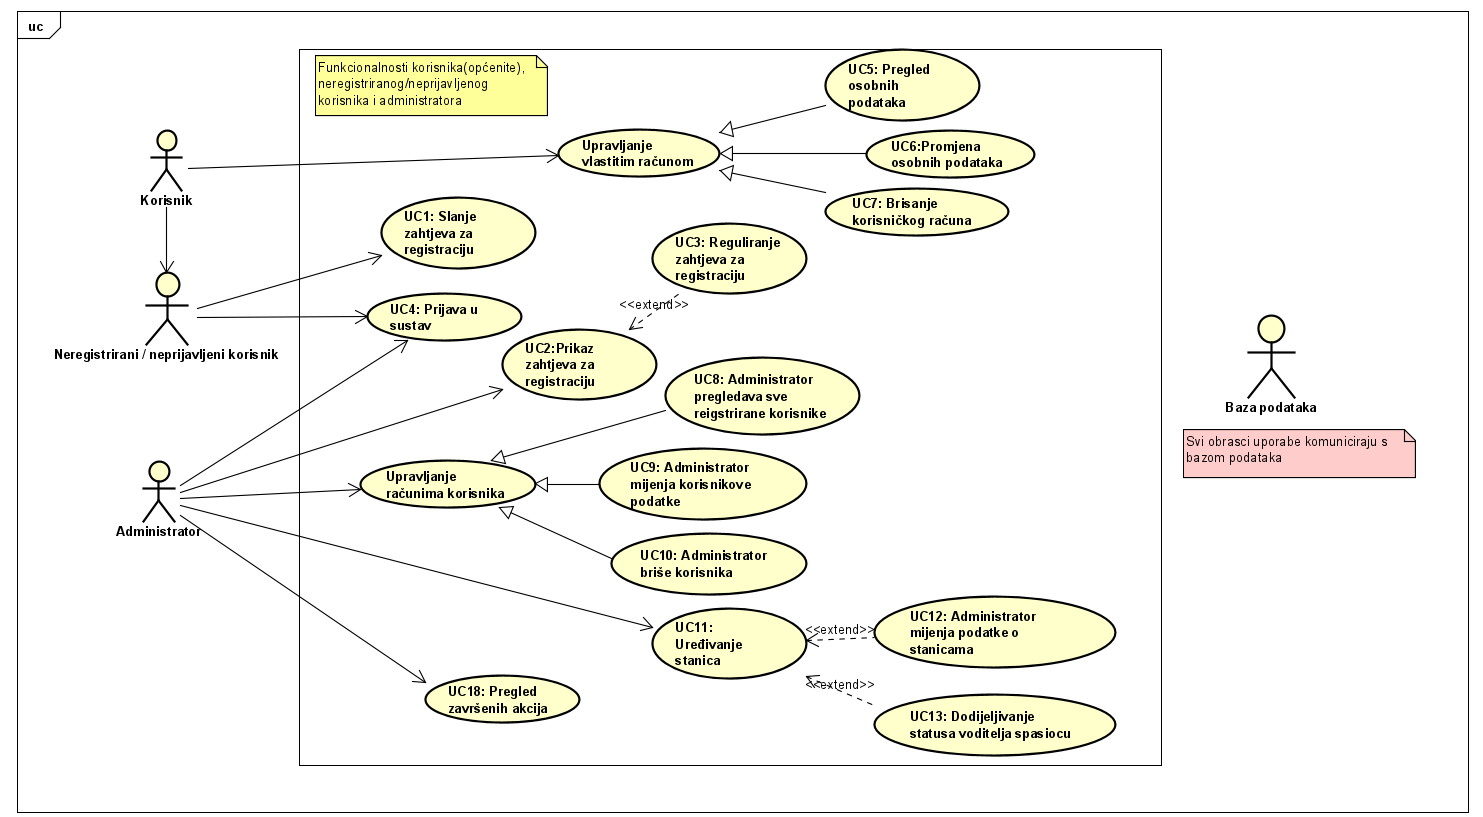
\includegraphics[width=\textwidth]{./slike/Korisnik,Administrator.png}
					\caption{Dijagram obrasca uporabe, funkcionalnost korisnika i administratora}
				
				\end{figure}
				
				\begin{figure}[h!]
					\centering
					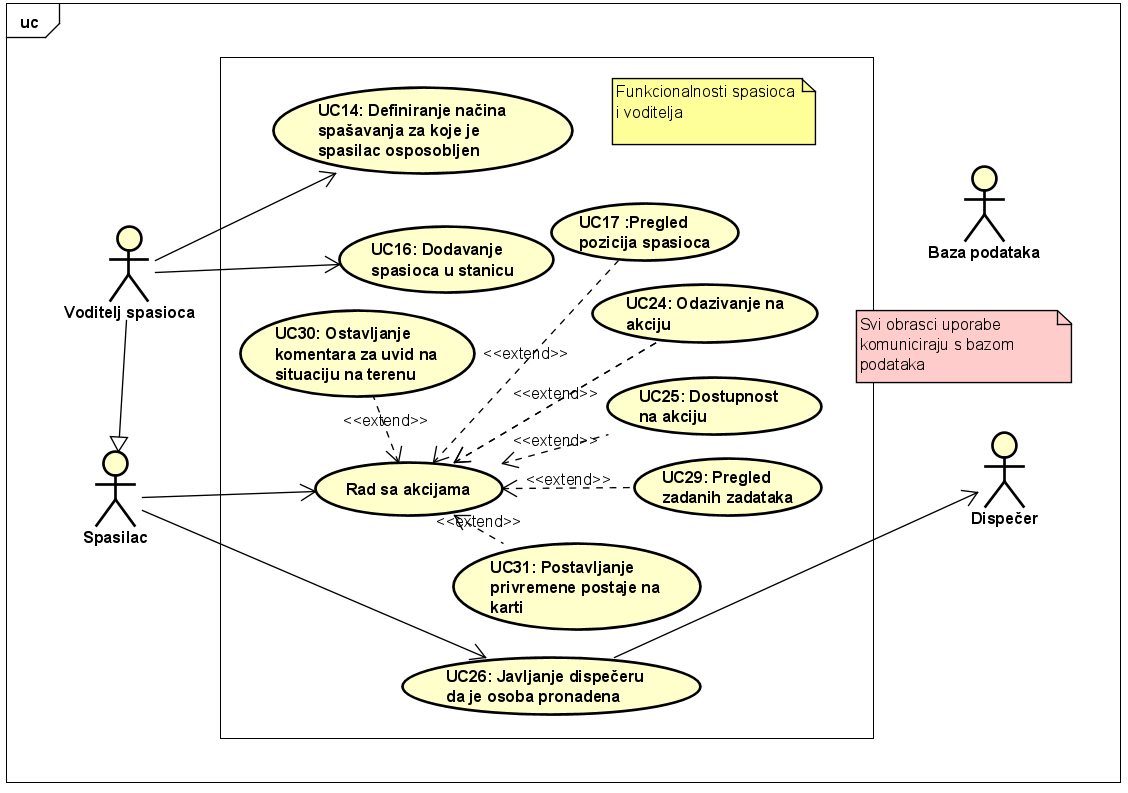
\includegraphics[width=\textwidth]{./slike/Spasioci.png}
					\caption{Dijagram obrasca uporabe, funkcionalnost spasioca}
					
				\end{figure}
				
				\begin{figure}[h!]
					\centering
					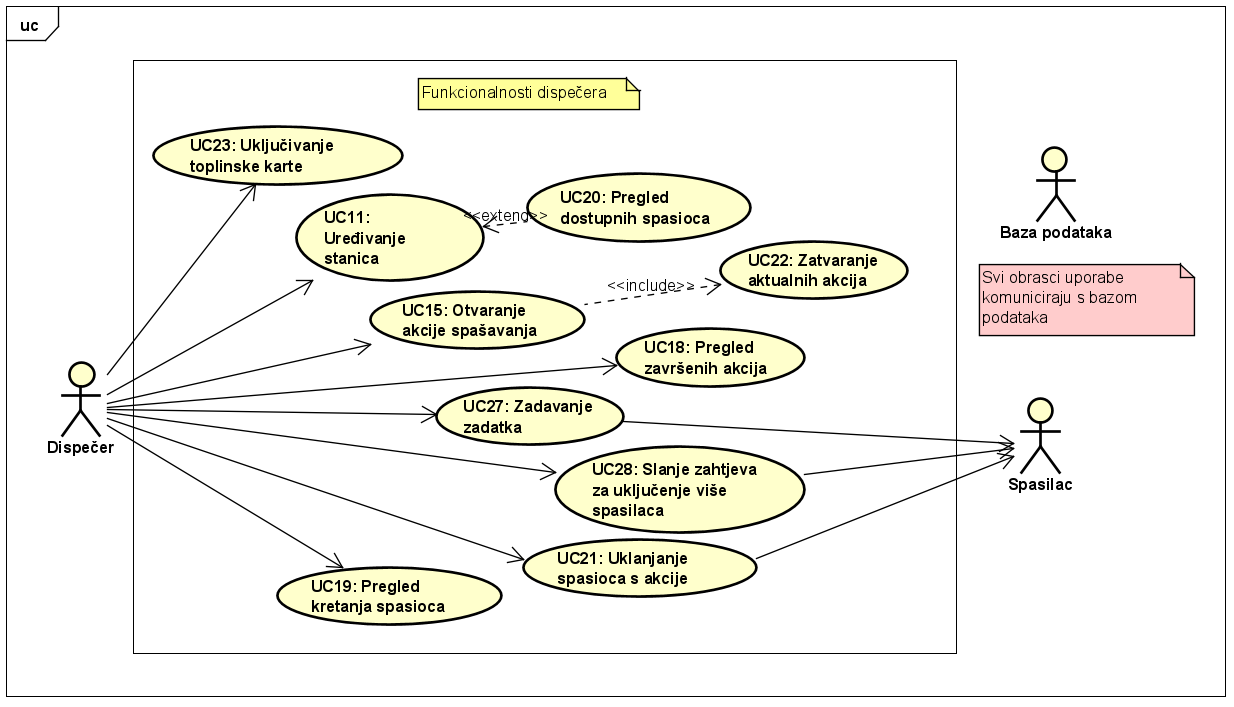
\includegraphics[width=\textwidth]{./slike/Dispecer.png}
					\caption{Dijagram obrasca uporabe, funkcionalnost dispečera}
					
				\end{figure}
			
				\cleardoublepage
				
			\subsection{Sekvencijski dijagrami}
			\begin{packed_item}
				
				
				\item \textbf{Obrazac uporabe UC15 $-$ Otvaranje akcije spašavanja}
				\\
				\item[] \begin{packed_item}
					{Dispečer dobiva poziv za pomoć (vanjska prijava).Upisuje podatke o nestaloj osobi i području na kojem se potraga treba odvijati. Nakon toga, dispečer šalje zahtjev za traženje dostupnih spasilaca čime akcija započinje. Spasioci se ovisno o raspoloživosti javljaju za sudjelovanje u akciji, a dispečer ima pregled svih osoba koje sudjeluju u akciji. U slučaju da se javi prevelik broj spasioca, dispečer ih može (ali ne mora) ukloniti iz akcije. Ako nema dovoljno spasioca, dispečer može poslati zahtjev za uključenje još spasioca u aktivnu akciju spašavanja.}
					
					\begin{figure}[h!]
						\centering
						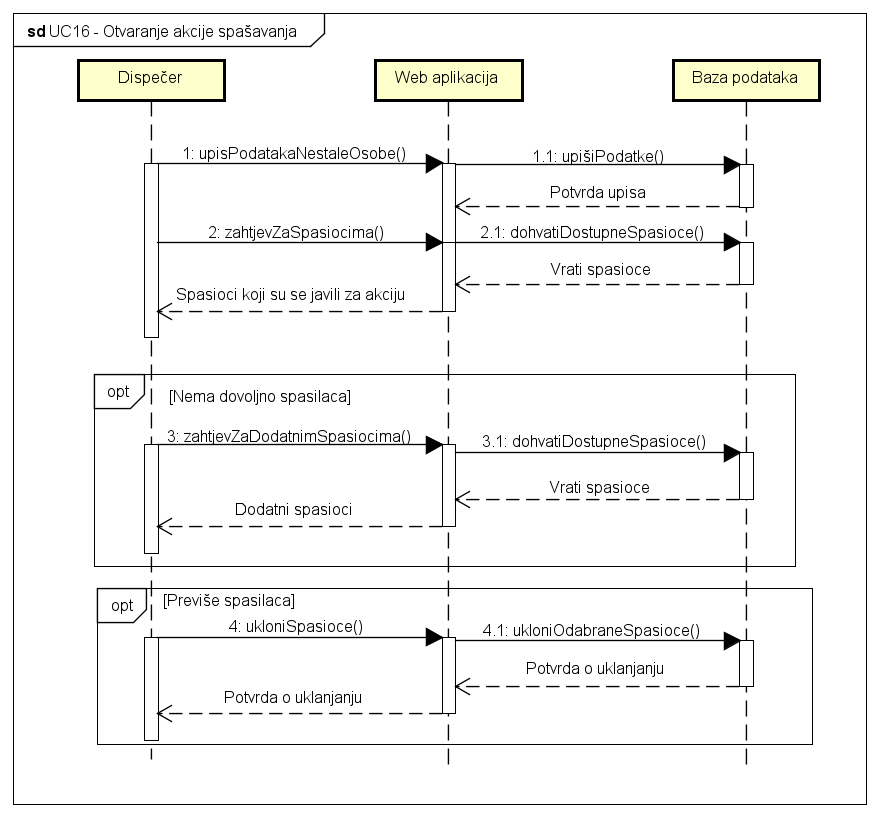
\includegraphics[width=\textwidth]{./slike/UC15.png}
						\caption{Sekvencijski dijagram za UC15}
						
					\end{figure}
					\eject
				\end{packed_item}
				\newpage
					
				\item \textbf{Obrazac uporabe UC24 $-$ Odazivanje na akciju}
				\\
				\item[] \begin{packed_item}
					{Spasilac dobiva obavijest o novoj akciji spašavanja. Ako ima mogućnosti sudjelovati, šalje zahtjev za pridruživanje timu za spašavanje. U slučaju da je osposobljen sudjelovati u toj akciji njegov zahtjev se prihvaća, a u protivnom biva odbijen.Ako je već aktivan na nekoj drugoj akciji, uklanja ga se sa stare akcije i dodaje u željenu akciju spašavanja.}
					
					\begin{figure}[h!]
						\centering
						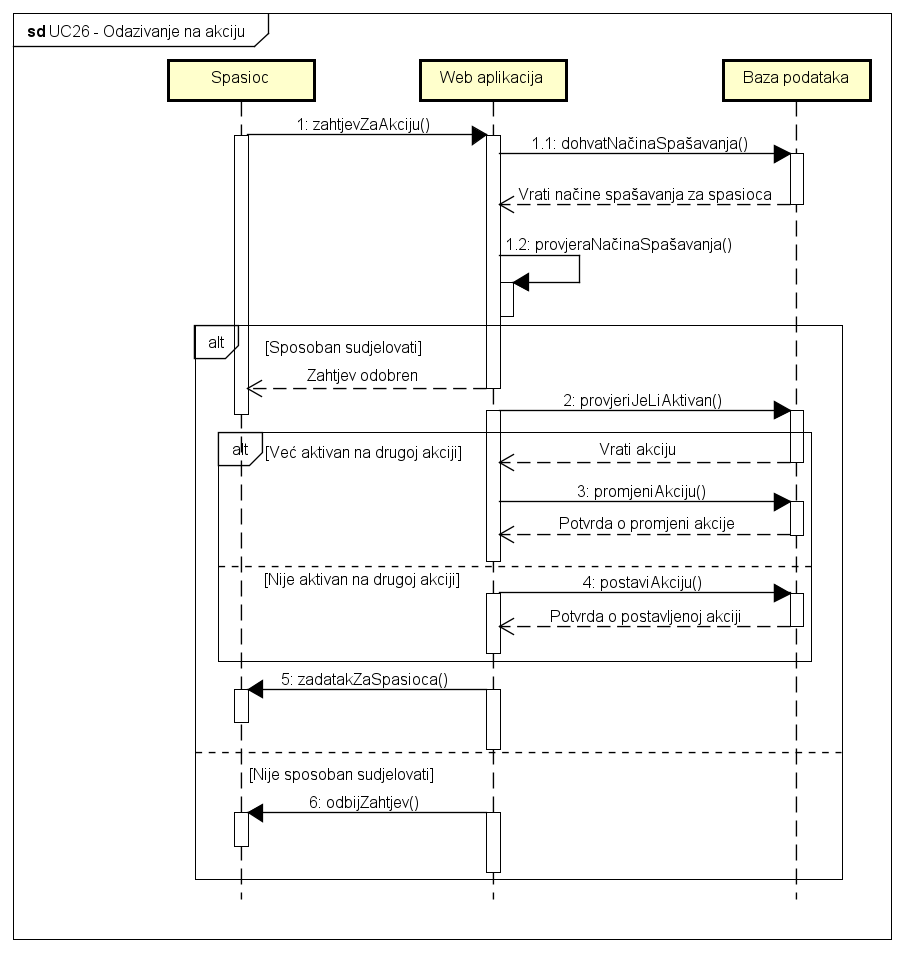
\includegraphics[width=\textwidth]{./slike/UC24.png}
						\caption{Sekvencijski dijagram za UC24}
						
					\end{figure}
					\eject
				\end{packed_item}
				\newpage
					
					
				\item \textbf{Obrazac uporabe UC27 $-$ Zadavanje zadatka}
				\\
				\item[] \begin{packed_item}
					{Dispečer spasiocima na aktivnoj akciji zadaje pojedinačne zadatke. Oni mogu biti: prođi određenom rutom, dođi do lokacije, postavi privremenu postaju ili osvježi zalihe u privremenoj postaji. Ako smatra potrebnim, dispečer može uz zadatak dodati i komentar.}
					
					\begin{figure}[h!]
						\centering
						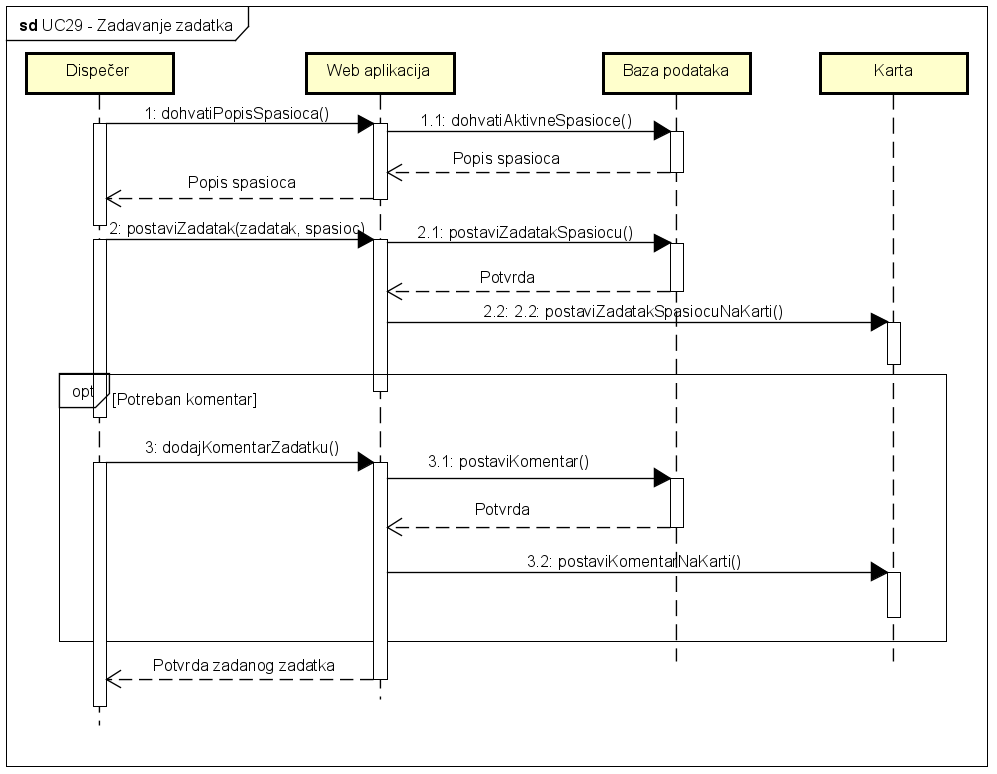
\includegraphics[width=\textwidth]{./slike/UC27.png}
						\caption{Sekvencijski dijagram za UC27}
						
					\end{figure}
					\eject
					
				\end{packed_item}
				\eject
			\end{packed_item}
			\newpage

	
		\section{Ostali zahtjevi\\}
		
		\begin{packed_item}
			
			\item Aplikacija mora omogućiti rad više korisnika u stvarnom vremenu
			\item Korisničko sučelje i sustav moraju podržavati hrvatsku abecedu
			\item Sustav treba biti implementiran kao web aplikacija dostupna svim korisnicima s javnog servisa
			\item Web aplikacija se će biti implementirana koristeći \textit{React} i \textit{Spring Boot framework}
			\item Sustav mora biti lak za održavanje i nadogradnju
			\item Neispravno korištenje aplikacije ne smije narušiti funkcionalnosti i rad sustava
			\item Izvršavanje dijela programa u kojem se pristupa bazi podataka ne smije trajati duže od nekoliko sekundi
			\item Sustav ne smije dozvoliti prikaz informacija korisnicima koji nisu ovlašteni da ih pregledavaju
			\item Sustav ne smije omogućiti korisnicima da obavljaju nedozvoljene operacije nad bazom podataka
			
		\end{packed_item}
			 
			 
			 
	